\chapter{Analisis}

\section{Mesin Navigasi KIRI}

\subsection{Mekanisme Penarikan}

Untuk mendukung integrasi data antara Peta Angkutan Umum dan KIRI, diperlukan adanya penarikan secara berkala terhadap Peta Angkutan Umum oleh KIRI. Ada dua alternatif metode yang dipertimbangkan sebagai mekanisme penarikan data ini:

\begin{description}
	\item \textbf{Metode \textit{realtime}} mendeteksi setiap perubahan yang terjadi pada data Peta Angkutan Umum, dan langsung memberi notifikasi kepada KIRI untuk mengambil ulang data yang berubah dari Peta Angkutan Umum
	\item \textbf{Metode \textit{polling}} di mana KIRI akan mengambil data secara berkala dari Peta Angkutan Umum, sehingga akan terdapat jeda antara perubahan data dan terbaharuinya data KIRI.
\end{description}

Dari kedua metode tersebut, metode \textit{polling} dipilih dengan alasan-alasan sebagai berikut:

\begin{itemize}
	\item \textbf{Lebih sedikit perubahan} Peta Angkutan Umum menggunakan protokol HTTP yang bersifat \textit{conectionless}, sehingga secara alami akan menunggu perintah dari \textit{client}, alih-alih secara aktif memberi notifikasi kepada \textit{client}. Jika menggunakan metode \textit{polling}, KIRI dapat memanfaatkan protokol \textit{Transportation Detail} yang sudah dimiliki oleh Peta Angkutan Umum.
	\item \textbf{Mengurangi kebutuhan prosesor} Rute pada KIRI dimodelkan dalam bentuk graf, dan sebelum dapat digunakan untuk pencarian graf ini harus dikonstruksi terlebih dahulu. Akibat besarnya data yang digunakan, konstruksi ini akan memakan waktu (kurang lebih 30 detik). Dengan menggunakan metode \textit{realtime}, setiap perubahan data pada kiri.web.id akan mengakibatkan graf ini harus direkonstruksi ulang. Dengan menggunakan metode \textit{polling}, penarikan data dan rekonstruksi graf dapat diatur sedemikian sehingga dilakukan pada saat pengguna sedang tidak aktif.
	\item \textbf{Urgensi Perbaikan Data} Urgensi perbaikan data tidak terlalu tinggi untuk KIRI (jika dibandingkan dengan perubahan harga saham, \textit{realtime GPS monitoring}, dll) sehingga penarikan tidak perlu dilakukan terlalu sering.
\end{itemize}

Ditetapkan penggunaan metode \textit{polling} selama 24 jam sekali, dan dipilih waktu 0.30 (setengah jam setelah tengah malam) untuk melakukan \textit{polling}. Penetapan waktu ini mempertimbangkan sedikitnya penggunaan KIRI pada saat tengah malam. Jeda setengah jam dilakukan untuk memberikan toleransi terhadap perbedaan waktu komputer beberapa detik, yang mungkin memberikan masalah pada tanggal sistem. 

\subsection{Penyimpanan Data}

Penyimpanan data diusahakan untuk meminimalisir perubahan serta menjaga kompatibilitas dengan versi sebelumnya. Seperti yang telah dibahas pada bab 2, mesin navigasi KIRI menggunakan berkas \texttt{tracks.conf} sebagai jembatan dari basis data menuju mesin navigasi. Berkas inilah yang akan dikonstruksi menjadi graf oleh kelas \texttt{Worker}. Peneliti memutuskan untuk tidak mengubah format dari berkas ini, melainkan melakukan modifikasi pada basis data.

Pada basis data, tetap diusahakan untuk meminimalisir perubahan. Dari struktur tabel \texttt{tracks} yang digunakan, diidentifikasi bahwa kolom `internalInfo` tidak digunakan dalam perhitungan (tidak berpengaruh pada konstruksi graf). Oleh sebab itu, kolom ini menjadi kandidat untuk disisipkan informasi terkait dengan penarikan data dari Peta Angkutan Umum. Adapun informasi yang harus disimpan adalah:

\begin{itemize}
	\item Penanda bahwa rute ini ditarik dari Peta Angkutan Umum
	\item Kode yang mengacu pada basis data Peta Angkutan Umum, dalam hal ini \texttt{id}.
\end{itemize}

%Peneliti memutuskan untuk menyimpan kedua informasi tersebut dalam kolom \texttt{internalInfo}, dengan format "angkotwebid:\textit{id}". Dengan cara ini, trayek yang memiliki \texttt{internalInfo} diawali dengan "angkotwebid:" akan diproses lebih lanjut dengan menarik data dari Peta Angkutan Umum. Penarikan data dilakukan dengan mendapatkan \textit{id} yang berada setelah simbol ":", dan menariknya di Peta Angkutan Umum dengan perintah \textit{Transportation Detail}. Sebagai contoh, jika ditemukan data dengan \texttt{internalInfo} bernilai "angkotwebid:1", akan ditarik data rute dari alamat \url{https://angkot.web.id}. Rute yang didapat tersebut kemudian akan dimasukkan ke dalam basis data pada kolom \texttt{geodata}.

\subsection{Analisis Aplikasi}

Pada penelitian ini, mesin navigasi KIRI dimodifikasi dengan menambahkan dua kelas baru, yaitu kelas \texttt{DataPuller} yang difungsikan sebagai penarik data dari Peta Angkutan Umum, serta kelas \texttt{DataPullerException} untuk mencatat kesalahan pada saat menarik data dari Peta Angkutan Umum. Kelas-kelas yang baru serta yang lama digambarkan pada diagram kelas di gambar \ref{fig:3_diagram_kelas_sistem_usulan}.

\begin{figure}
	\centering
	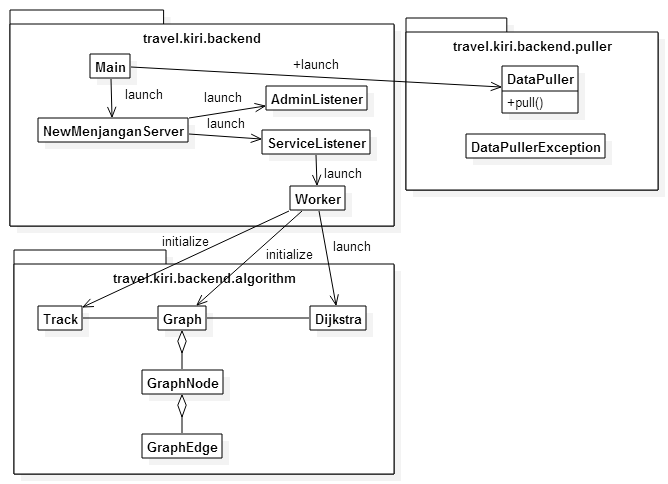
\includegraphics[scale=0.5]{Gambar/3_diagram_kelas_sistem_usulan}
	\caption{Diagram Kelas Sistem Usulan (Tahap Analisis)} 
	\label{fig:3_diagram_kelas_sistem_usulan}
\end{figure}

\section{Peta Angkutan Umum}

Pada dasarnya Peta Angkutan Umum tidak diperlukan adanya perubahan, karena KIRI dapat memanfaatkan protokol \textit{transportartion detail}. Namun, untuk keperluan optimasi, ada sedikit perubahan yang dijelaskan pada subbab berikutnya.

\section{Optimasi}

Dengan mekanisme yang sudah dijelaskan di subbab sebelumnya, data pada KIRI dapat tersinkronisasi dengan Peta Angkutan Umum. Namun, mekanisme tersebut dirasa tidak optimal. Setiap pukul 0.30, KIRI akan menarik ke-33 rute angkot yang dicatat pada Peta Angkutan Umum, terlepas dari apakah ada perubahan pada rute angkot atau tidak. Walaupun hanya menarik 33 rute dan dilakukan pada jam tidak sibuk, peneliti merasa optimasi tetap dibutuhkan sehingga solusi ini skalabel.

Mekanisme \textit{Transportation List} maupun \textit{Transportation Detail} pada Peta Angkutan Umum memberikan informasi \textit{updated} yang menunjukkan waktu terakhir rute ini diperbaharui. Pada saat menarik data dari Peta Angkutan Umum, informasi ini dapat dicatat dan disimpan pada basis data, untuk dibandingkan pada kesempatan berikutnya. Jika informasi \textit{updated} yang terdapat pada basis data sama atau lebih baru dibandingan dengan yang didapat dari Peta Angkutan Umum, maka tidak diperlukan adanya penarikan rute dari Peta Angkutan Umum. Adapun informasi yang dicatat pada basis data KIRI menjadi sebagai berikut (informasi baru hasil optimasi \textbf{dicetak tebal}):

\begin{itemize}
	\item Penanda bahwa rute ini ditarik dari Peta Angkutan Umum
	\item Kode yang mengacu pada basis data Peta Angkutan Umum, dalam hal ini \texttt{id}.
	\item \textbf{Waktu terakhir rute ini berubah pada Peta Angkutan Umum}
\end{itemize}

Perlu dicatat pula bahwa tidak semua data trayek di Peta Angkutan Umum akan diintegrasikan dengan KIRI. Oleh karena itu, dibutuhkan sedikit perubahan pada Peta Angkutan Umum, sehingga KIRI dapat menarik informasi untuk rute-rute yang dibutuhkan saja. Detail dari perubahan ini akan dijelaskan pada bab berikutnya.